\documentclass{beamer}

\usepackage[ngerman]{babel}
\usepackage{graphicx}
\usepackage{hyperref}


% Example here:
% https://github.com/josephwright/beamer/blob/main/doc/solutions/conference-talks/conference-ornate-20min.de.tex

\mode<presentation>
{
    \usetheme{Singapore}
%\usetheme{AnnArbor}
%\usecolortheme{beaver}
}

\title{Kolloquium Feinspezifikation}
\subtitle{SEP WS 2021/2022}

%\titlegraphic{
\includegraphics[width=5cm]{../../docs/Pflichtenheft/graphics/LasEs-logo}}

\date{\small 30. November 2021}
\logo{
\includegraphics[width=1.5cm]{../../docs/Pflichtenheft/graphics/LasEs-logo}}

\author{\textbf{Team 2} \\ \small {Johann Schicho, Stefanie Gürster, Thomas Kirz,\\ Johannes Garstenauer, Sebastian Vogt} \\ \vspace{0.5cm}\emph{Phasenleiter: Johannes Garstenauer}\normalsize}


\begin{document}

    \begin{frame}{Start}
        \titlepage
    \end{frame}

%    \section{Änderungen}
%    \begin{frame}{Evolution}
%        Vereinfachungen \& Übersichtlickeit
%        (Um das Produkt für Sie besser zu gestalten haben wir einige Verbesserungen vorgenommen:)
%        \begin{itemize}
%            \item Neue Pakete zur Übersichtlichkeit und Einhaltung der selbstdefinierten Paketfunktionen
%            z.B. persistence.internals zum Zugriff auf Konfig \& Res.Bundles, da repositories für entitäten gedacht sind.
%            \item Verwendung des Standardlogger
%            \item Facelets wurden zusammengelegt (z.B. Ansicht und Bearbeitung einer Einreichung)
%            \item Pagination DTOs wurden simplifiziert
%       \end{itemize}
%        Verinfachungen machen die Implementation weniger zeitaufwendig.
%        Übersichtlichkeit macht die Planung leíchter.
%       Somit ist das Produkt günstiger für Sie.
%   \end{frame}


    \section{Struktur}
    \begin{frame}{Ordnerstruktur}
        %todo nebeneinander & lesbar
        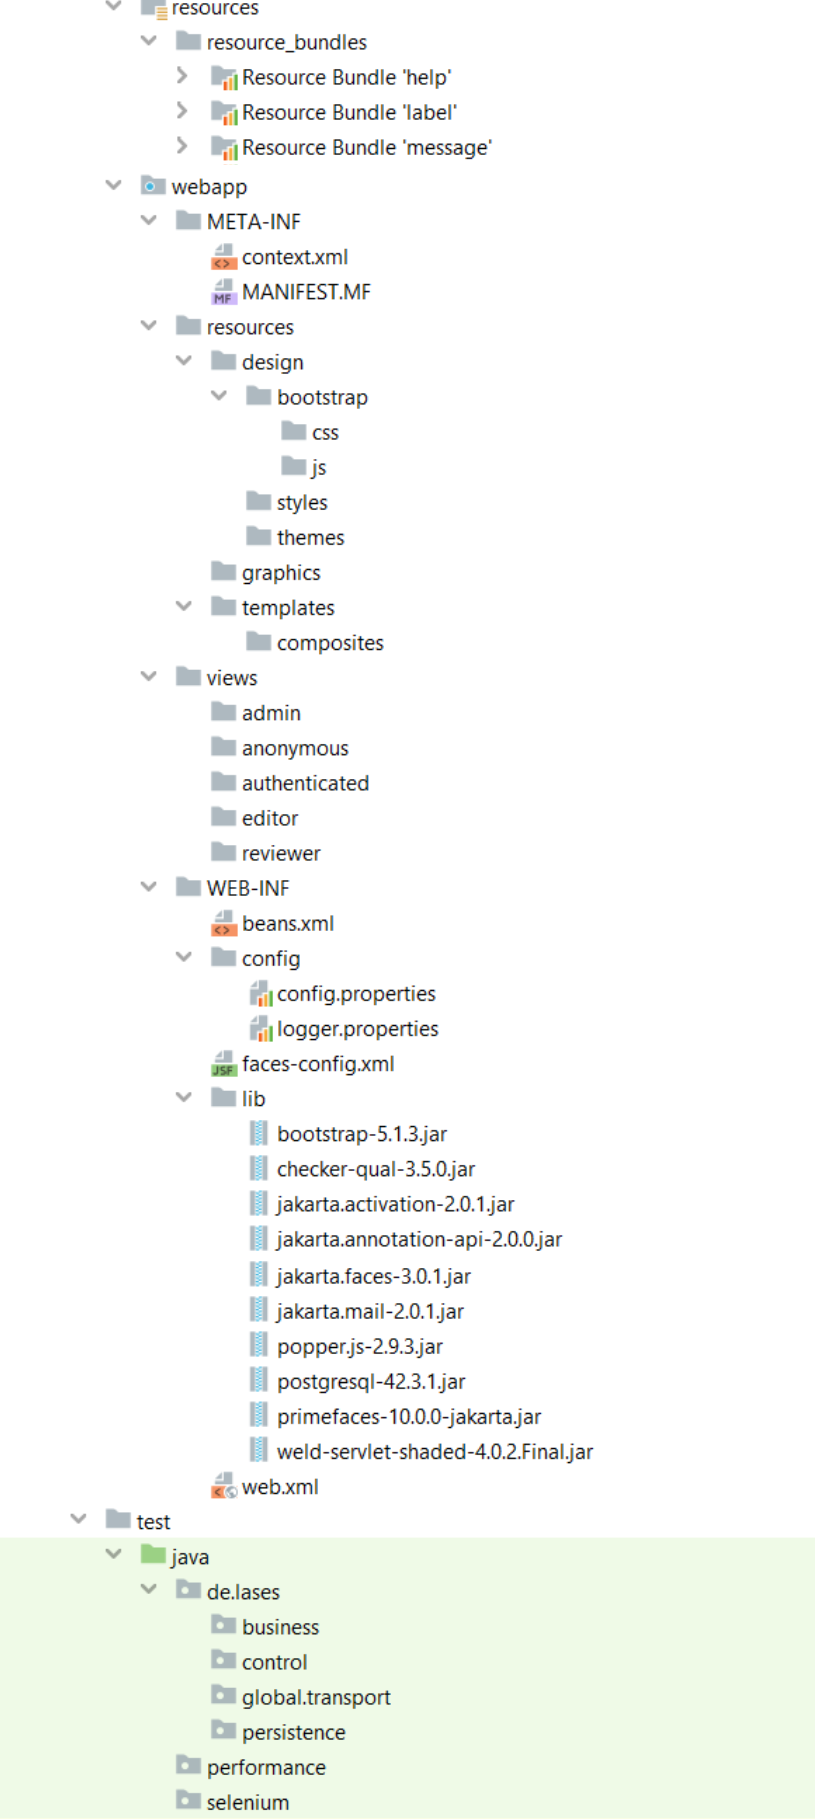
\includegraphics[height=0.9\textheight]{graphics/w2_folder_final_smaller}
    \end{frame}


    \begin{frame}{Paketdiagramm}
        \centering
        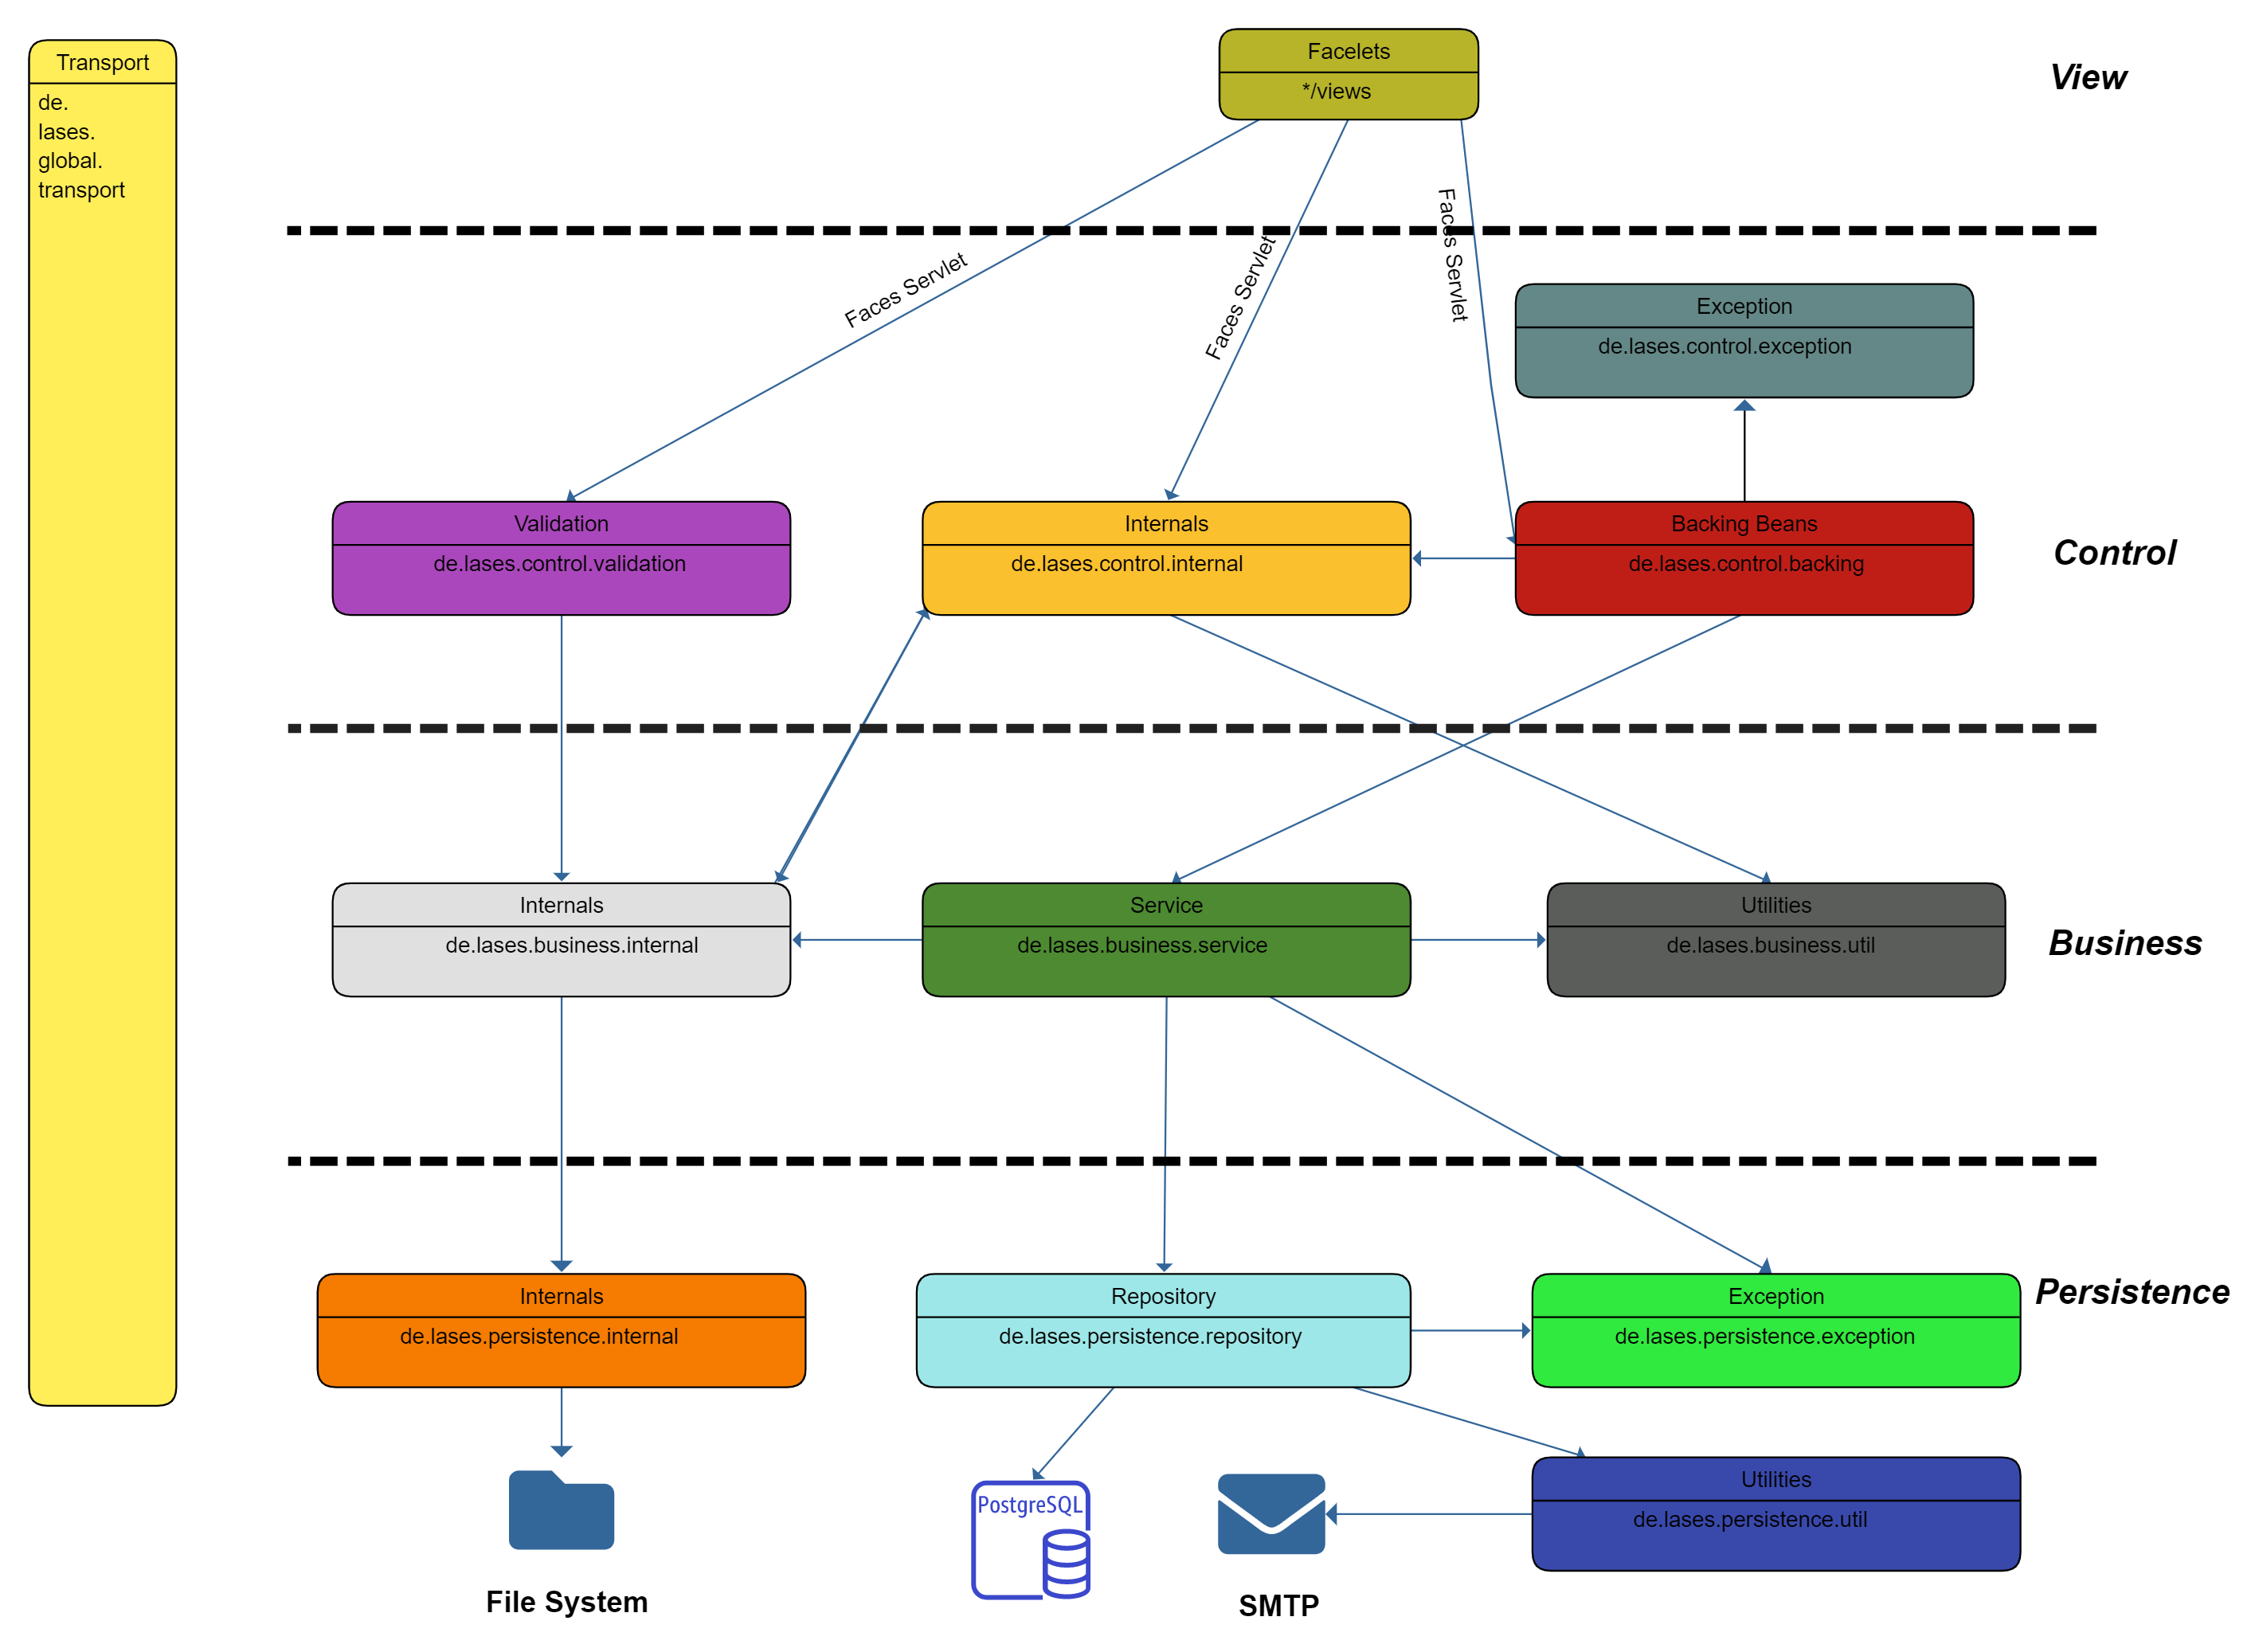
\includegraphics[height=0.8\textheight]{graphics/Paketdiagramm (15)}
        % Größtenteils gleichgeblieben. Änderungen aus Punkt 1 wurden übernommen.
        % Wir haben besonders darauf geachtet:
        % Klare Trennung der Schichten, verständliche Interfaces und v.a. schwache Kopplung!
        %  Wir garantieren: Sie können diese Anwendung noch sehr lange verwenden,
        % alle schichtenspezifischen Technolgien wie z.B. die PostGres-Datenbank
        % oder Facelets von JSF sind komplett und problemlos austauschbar!
    \end{frame}


    \section{Datenfluss}
    % Nun möchte ich Ihnen Beispielhaft zeigen, wie diese Architektur im Detail zusammenspielt.
    % Ausschnitthaftes Beispiel des Aufbaus der Seite zur Einreichung einer Darstellung
    % mit Exkursen anhand derer typische Klassenspezifikationen klar werden sollen.
    % Beginnen wir mit dem notwendigen Facelet.

    %todo hier überscichtseite für allg. kommentare vllt submission mockup
    \begin{frame}{\textbf{Typisches Facelet:} submission.xhtml}
        %Ziel: Welche Elemente verwenden wir:
        %-> Personalisierte Seiten für bestimmte Nutzerrollen
        \textbf{Element:} 'rendered='
        \newline\newline
        \centering
        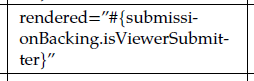
\includegraphics[height=0.3\textheight]{graphics/facelet/fac_rendered}
    \end{frame}
    \begin{frame}{\textbf{Typisches Facelet:} submission.xhtml}
        %-> Zur Eingabevalidation erstens
        %-> mit message aus RessourceBundle
        \textbf{Element:}'required=' + 'requiredMessage='
        \newline\newline
        \centering
        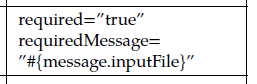
\includegraphics[height=0.3\textheight]{graphics/facelet/fac_required}
    \end{frame}
    \begin{frame}{\textbf{Typisches Facelet:} submission.xhtml}
        %-> Zur Eingabevalidation zweitens
        %todo switch DateInFutureTimeValidator
        \textbf{Element:} Validatoren
        \newline\newline
        \centering
        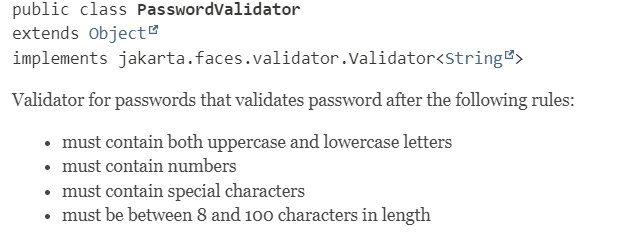
\includegraphics[height=0.4\textheight]{graphics/facelet/doc_validator}
    \end{frame}
    \begin{frame}{\textbf{Typisches Facelet:} submission.xhtml}
        % Generische Pagination, die mit jedem DTO befüllbar ist
        % abstrakte Methode loaddata() mit welcher individuell und vielfältig
        % die Pagination für jeden Verwendung bestimmt werden kann
        \textbf{Element:} Pagination
        \newline\newline
        \centering
        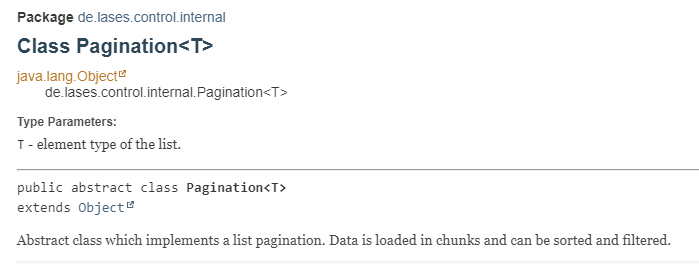
\includegraphics[height=0.5\textheight]{graphics/facelet/pagination/doc_pag}
    \end{frame}
    \begin{frame}{\textbf{Typisches Facelet:} submission.xhtml}
        % Abstrakte Methode loaddata() mit welcher individuell und vielfältig
        % die Pagination für jeden Verwendung bestimmt werden kann}
        \textbf{Element:} Pagination
        \newline\newline
        \centering
        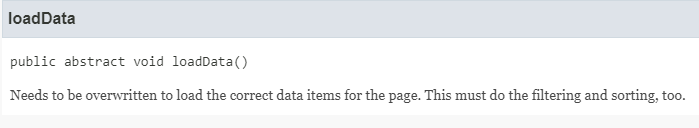
\includegraphics[height=0.2\textheight]{graphics/facelet/pagination/doc_loaddata}
    \end{frame}
    \begin{frame}{\textbf{Typisches Facelet:} submission.xhtml}
        % Außerdem ist unsere Pagination leistungsfähig und adaptierbar an persönlich Verwendung
        % durch hervorragende Sortierbarkeit und Filterbarkeit
        %-> Sie können ihr Produkt an Profis verkaufen, es ist für professionelle Verwendung geeignet
        \textbf{Element:} Pagination
        \newline\newline
        \centering
        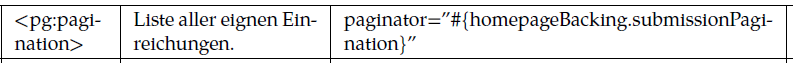
\includegraphics[height=0.1\textheight]{graphics/facelet/pagination/fac_pag}
        %todo falscher screenshot
    \end{frame}
    \begin{frame}{\textbf{Typisches Facelet:} submission.xhtml}
        % -> Der Aufbau der Daten die im Facelet angezeigt werden erfolgt folgendermaßen:
        % -> Erhalten der Id der Einreichung
        \textbf{Datenfluss:} <f:viewParam>
        \newline\newline
        \centering
        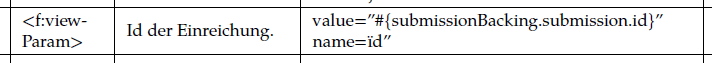
\includegraphics[height=0.1\textheight]{graphics/facelet/fac_viewParam}
    \end{frame}
    \begin{frame}{\textbf{Typisches Facelet:} submission.xhtml}
        % -> Dieses wird mithilfe eines Events validiert, sodass keine Korruption der URL möglich ist
        \textbf{Datenfluss:} <f:event>
        \newline\newline
        \centering
        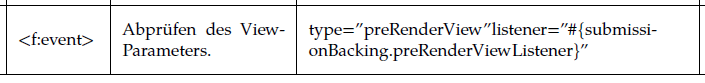
\includegraphics[height=0.1\textheight]{graphics/facelet/fac_event}
        %todo include doc bb methode
    \end{frame}
    \begin{frame}{\textbf{Typisches Facelet:} submission.xhtml}
        % -> Schließlich: Starten der onLoad() zum Befüllen der DTOs
        \textbf{Datenfluss:} <f:viewAction>
        \newline\newline
        \centering
        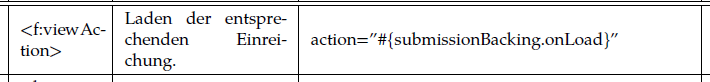
\includegraphics[height=0.1\textheight]{graphics/facelet/fac_onLoad}
    \end{frame}

    % Nun liegt die Arbeit beim zugehörigen Backing Bean.
    \begin{frame}{Typische Klasse \textbf{Kontrollschicht}: \emph{SubmissionBacking}}
        \centering
        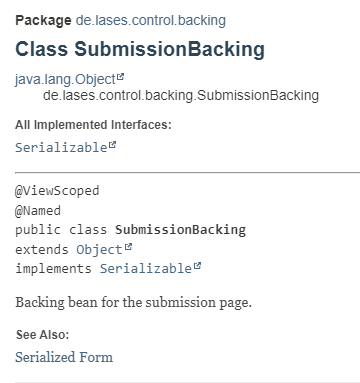
\includegraphics[height=0.7\textheight]{graphics/backing/doc_backing}
    \end{frame}
    \begin{frame}{Typische Klasse der \textbf{Kontrollschicht}: \emph{SubmissionBacking}}
        % Zuerst werden dessen nötige DTOs initalisiert
        % -> Instanziierung aller benötigten DTOs z.B.:
        %            -User mit ID aus Session
        %            -Submission
        \centering
        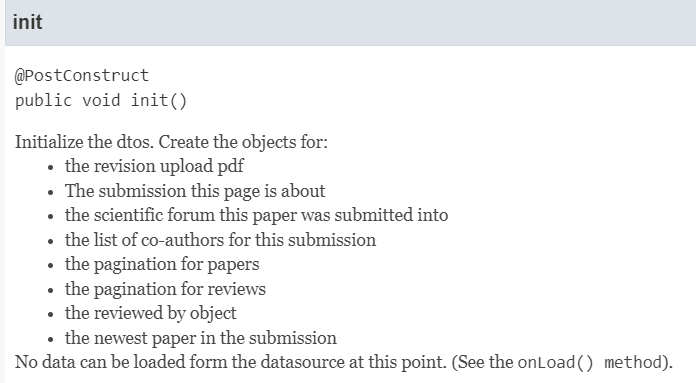
\includegraphics[height=0.6\textheight]{graphics/backing/doc_init}
    \end{frame}
    \begin{frame}{Typische Klasse \textbf{Kontrollschicht}: \emph{SubmissionBacking}}
        % Befüllen der DTOs mithilfe id aus <f:viewParam>
        % Getriggert durch vorheriges <f:viewAction>
        \centering
        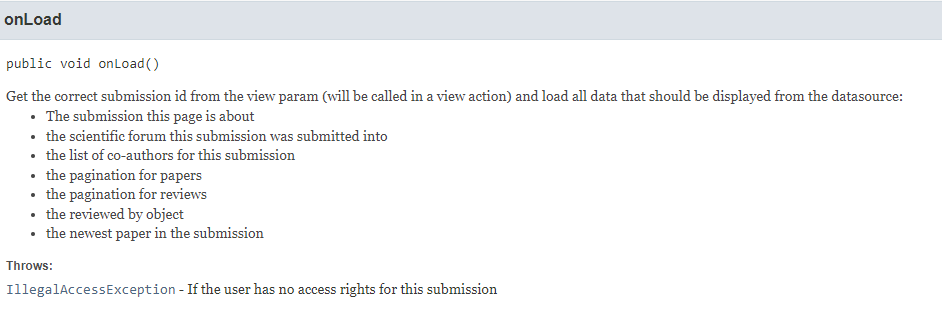
\includegraphics[height=0.5\textheight]{graphics/backing/doc_onLoad}
    \end{frame}

    \begin{frame}{Typische Klasse \textbf{Businessschicht}: \emph{SubmissionService}}
        % Für diese action-Methoden und für unser Beispiel die onLoad() benötigen wir nun Zugriff auf
        % die Daten und die Businesslogik, welche durch den SubmissionService zur Verfügung gestellt wird
        %todo hier besonders auf DTO-Spezifikation für Methoden eingehen
        \centering
        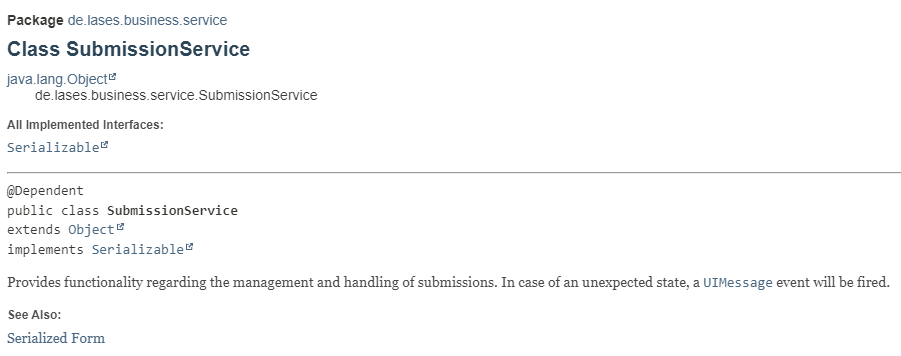
\includegraphics[height=0.5\textheight]{graphics/service/doc_service}
    \end{frame}
    \begin{frame}{Typische Klasse \textbf{Businessschicht}: \emph{SubmissionService}}
        % Für das Laden der DTOs wird ein get() benötigt.
        % Weiterhin angeboten werden jeweils immer die Methoden
        \centering
        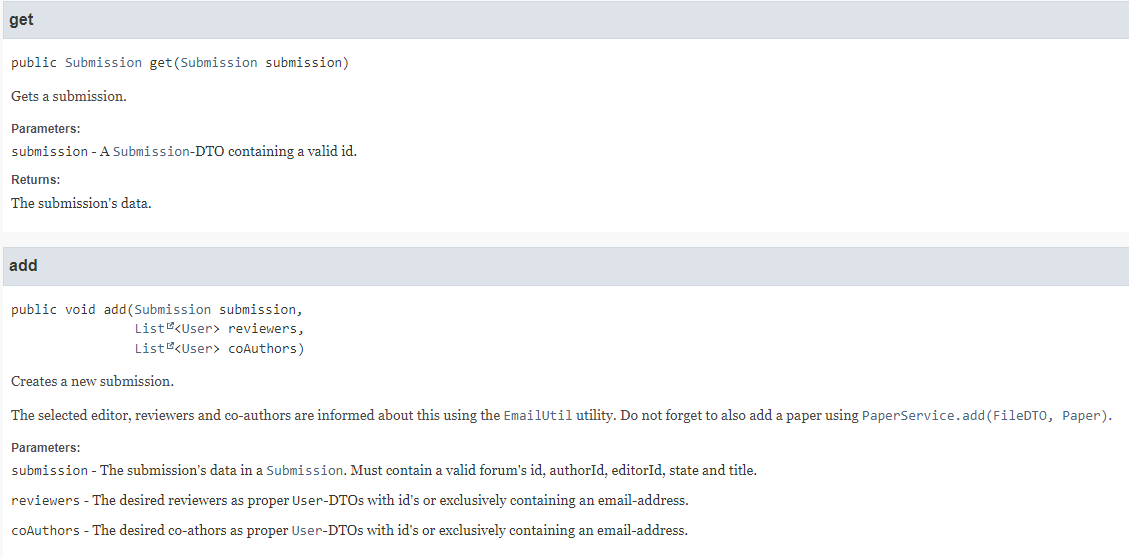
\includegraphics[height=0.6\textheight]{graphics/service/doc_get_add}
    \end{frame}
    \begin{frame}{Typische Klasse \textbf{Businessschicht}: \emph{SubmissionService}}
        %todo remove?
        \centering
        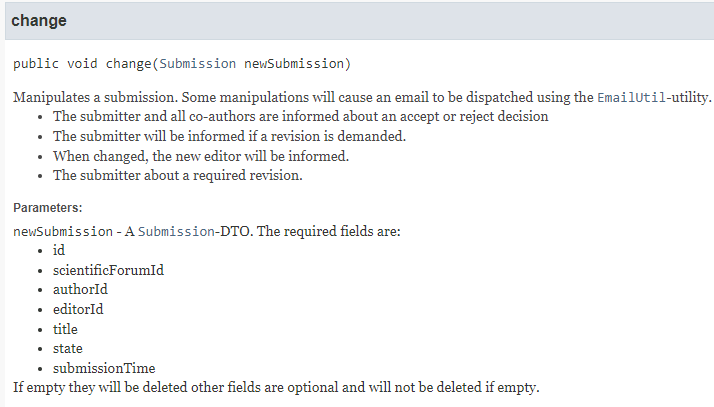
\includegraphics[height=0.6\textheight]{graphics/service/doc_change}
        %-> einheitliche und übersichtliche Interfaces:
        % Beachte: obwohl Methodensignatur selbe Parameter: verschiedene Anforderungen.
        % -> in javadoc spezifiziert
        % -> Ermöglicht Datenfluss ohne flache Parameter, gekapselt in DTOs
        % Hohe Überdeckung zu Persistenzschicht
    \end{frame}
    \begin{frame}{Typische Klasse \textbf{Businessschicht}: \emph{SubmissionService}}
        Event<UIMessage>\#fire()
        \centering
        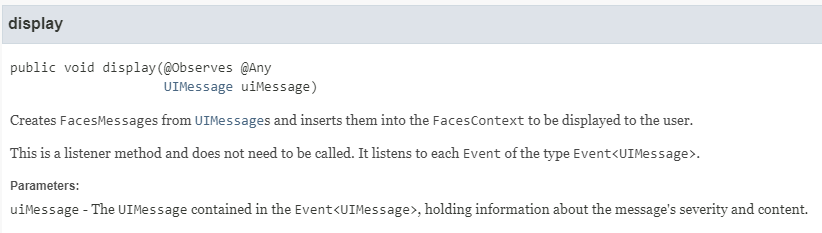
\includegraphics[height=0.3\textheight]{graphics/service/doc_uim}
        %todo hier besonders auf annotationen/listeners einegehn
        % informiert den Nutzer über fehlerhaften Zustand aus unteren Schichten und in der Geschäftslogik
        % werden zu FacesMessages umgewandelt
        % -> Vorteil der Modulariät und Vermeidung von Coderedundanzen
        % -> günstigeres Produkt für Sie!
    \end{frame}

    \begin{frame}{Typische Klasse \textbf{Persistenzschicht}: \emph{SubmissionRepository}}
        % Die benötigten Daten werden wiederum aus der Persistenzschicht geholt.
        % Genauer gesagt aus dem SubmissionRepository - einer typischen Klasse dieser Schicht.
        \centering
        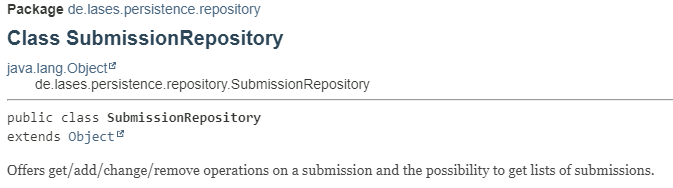
\includegraphics[height=0.3\textheight]{graphics/repo/doc_repo}
    \end{frame}
    \begin{frame}{Typische Klasse \textbf{Persistenzschicht}: \emph{SubmissionRepository}}
        % Enthält ausschließlich statische Methoden
        % Welche aus der DB DTOs erstellen und ausliefern.
        % Einheitlichketi -> Ebenfalls wieder get add change
        \centering
        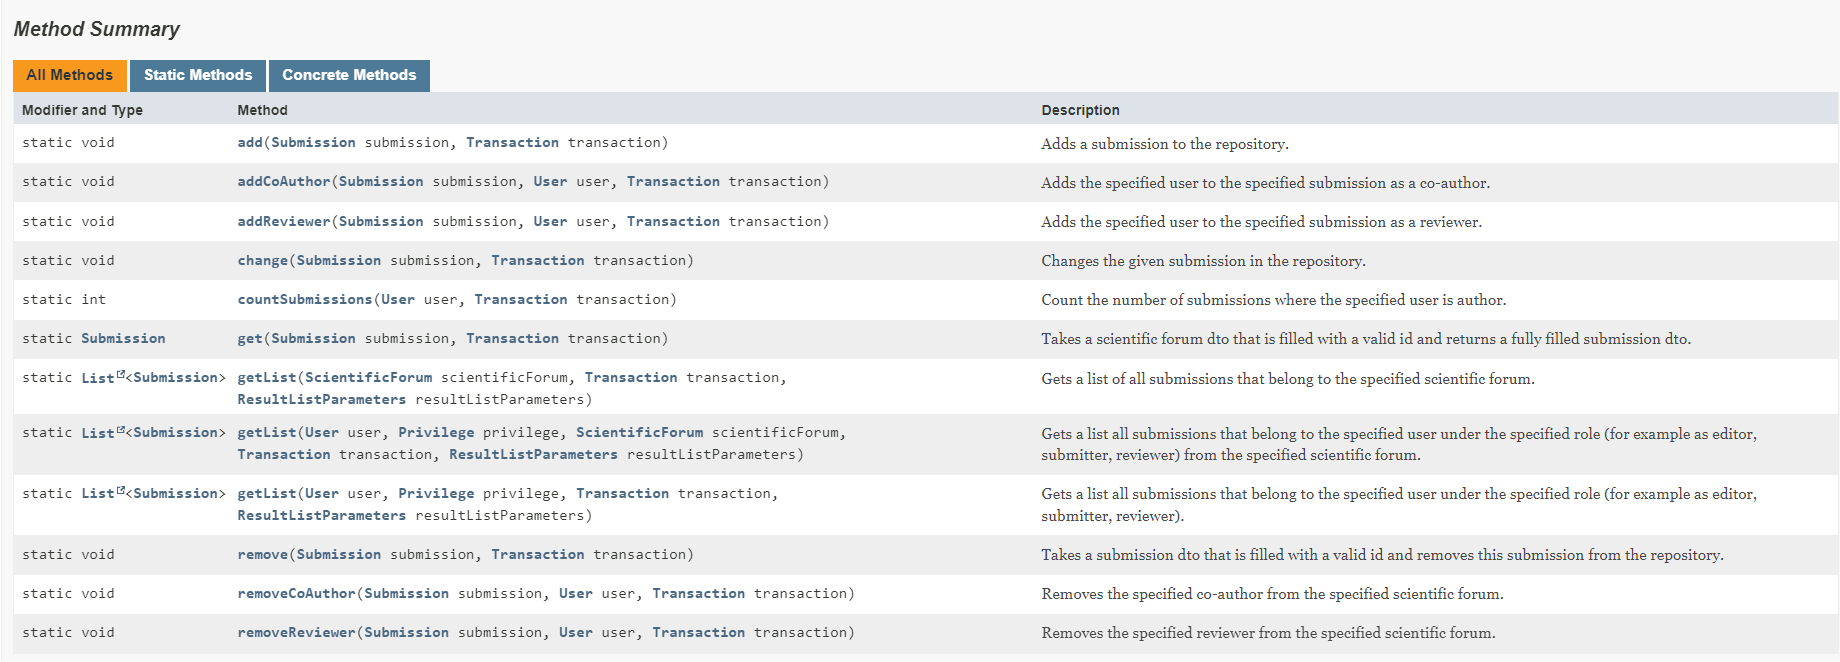
\includegraphics[height=0.5\textheight]{graphics/repo/doc_static}
    \end{frame}


    \section{Fehlerfall}
    % Wir haben checked Exceptions via Event-Architektur besprochen.
    % Was kann noch schiefgehen?
    % -> Race Conditions.
    % Wir verwenden serialisierte JDBC Transactions um diesen Vorzubegugen.
    % Wenn sie trzdm vorkommen, kapseln wir sie in semantische Exceptions
    % und starten dass Error-Handling
    % Hier ein Beispiel.
    \begin{frame}{Auftreten einer unchecked Exception}
        %todo weiter links
        \centering
        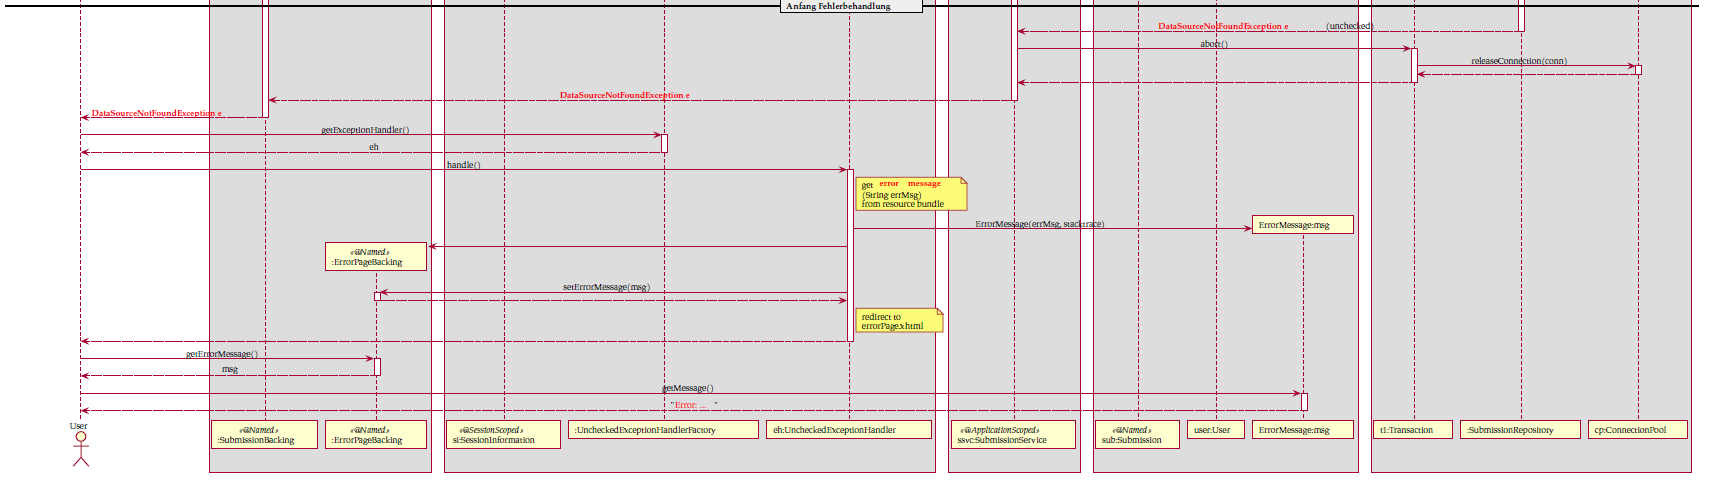
\includegraphics[height=0.4\textheight]{graphics/exc/seq_ex}
    \end{frame}
    \begin{frame}{Auftreten einer unchecked Exception}
        % Exception landet im FacesContext
        % Siehe Konstruktoren: wird mit Message befüllt
        \centering
        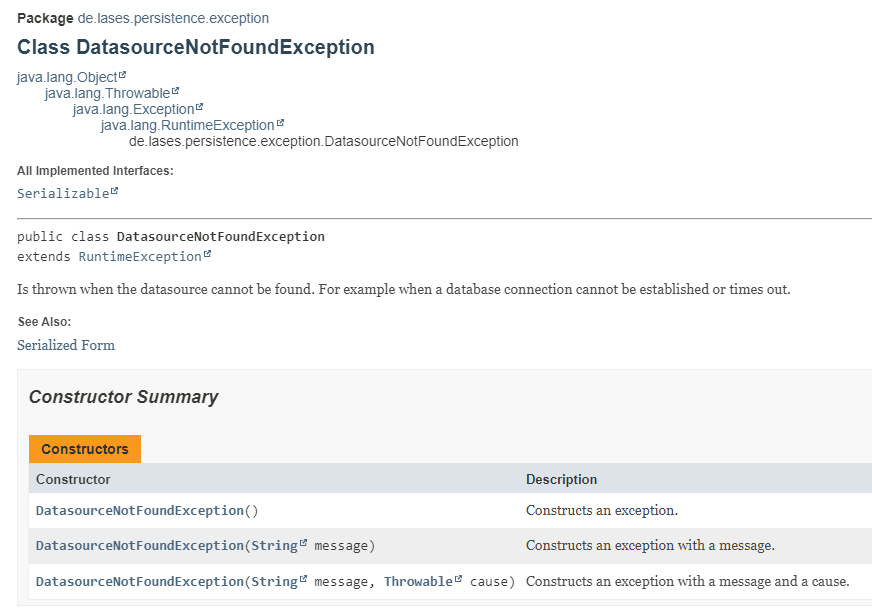
\includegraphics[height=0.6\textheight]{graphics/exc/doc_ex}
    \end{frame}
    \begin{frame}{UncheckedExceptionHandler}
        % Aufgegriffen vom UncheckedExceptionHandler
        % Leitet weiter auf ErrorPage
        \centering
        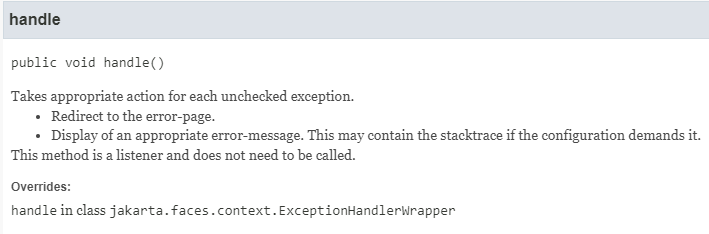
\includegraphics[height=0.4\textheight]{graphics/exc/doc_handle}
    \end{frame}
    \begin{frame}{UncheckedExceptionHandler}
        % Erstellt ErrorMsg und übergibt diese an das BB
        \centering
        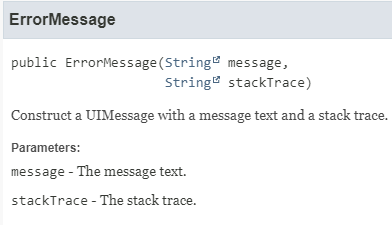
\includegraphics[height=0.5\textheight]{graphics/exc/doc_errormsg}
    \end{frame}
    \begin{frame}{UncheckedExceptionHandler}
        +
        % Falls development modus, dann zusätzlich der stacktrace
        \centering
        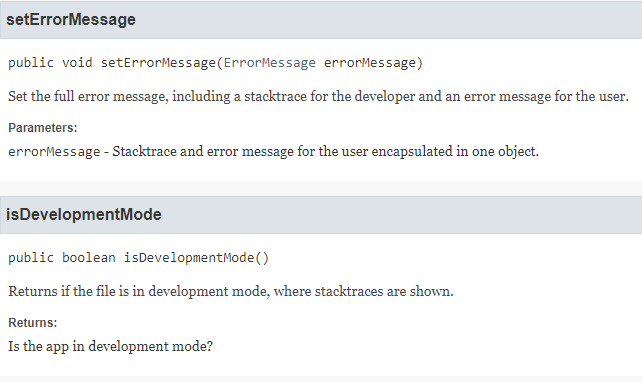
\includegraphics[height=0.6\textheight]{graphics/exc/doc_backing}
    \end{frame}

%\section{Session}
%\begin{frame}{Session}
%    \begin{itemize}
%        \item User\-DTO mit ID
    %-Immer nur mit ID? Wieso nur Id? (Auf mehr Daten kann man sich nicht verlassen, dass diese vorhanden sind: Minimum)
    %-Welche Elemente gerendert werden ist immer davon Abhängig wer eine bestimmte Seite sieht.
    %-Sicherheit: Hat diese Session Zugriff auf best. Seite?
    %- Wieso nicht mehr in Session (Privilege z.B.)
%        \pause
%        \item Locale zur Internationalisierbarkeit.
    %- Ist Locale abfragbar? Sparen wir uns hiermit Anfragen an den Browser?
%    \end{itemize}
%\end{frame}


    \section{Konfiguration}
    \begin{frame}{Allgemeine Konfiguration}
        %todo bild
        \begin{itemize}
            \item Validation
            \pause
            \item Entwicklungsmodus
            \pause
            \item Mail
            \pause
            \item Datenbank
        \end{itemize}
    \end{frame}

    \begin{frame}{Loggerkonfiguration}
        \begin{itemize}
            \item Konsolenlogger
            \pause
            \item Filelogger
        \end{itemize}
    \end{frame}


    \section{Libraries}
    \begin{frame}{Basis}
        \begin{itemize}
            \item Mojarra v3.0.1
            \item JBoss Weld v4.0.2
            \item PostGreSQL JDBC v42.3.1
            \item Jakarta Mail API v2.0.1
        \end{itemize}
    \end{frame}

    \begin{frame}{Quality of Life}
        \begin{itemize}
            \item Primefaces v10.0.0
            \item Bootstrap v5.1.3
        \end{itemize}
    \end{frame}

    \begin{frame}{Testing}
        \begin{itemize}
            \item JUnit v5.8.1
            \item Mockito v4.0.0
            \item Selenium v4.0.0
        \end{itemize}
    \end{frame}


    \section{Diskussion}
    \begin{frame}{Diskussion}
        \centering
        
\includegraphics[width=0.7\linewidth]{../../docs/Pflichtenheft/graphics/LasEs-logo}
    \end{frame}

\end{document}
